% Part: model-theory
% Chapter: interpolation
% Section: separation

\documentclass[../../../include/open-logic-section]{subfiles}

\begin{document}

\olfileid{mod}{int}{sep}

\olsection{Pamisahan \printtoken{P}{sentence}}

Sadurunge nerusake bukti teorema interpolasi,
kita perlu nyiapake sawetara landhesan. Interpolan
kanggo $!A$ lan $!B$ yaiku !!a{sentence}~$!C$ kang
$!A \Entails !C$ lan $!C \Entails !B$.
Miturut kontraposisi, pratelan kang pungkasan
bener yen lan mung yen $\lnot !B \Entails \lnot
!C$. !!^a{sentence}~$!C$ kanthi sipat iki diarani
\emph{misahake} $!A$ lan $\lnot !B$.
Mula nggoleki interpolan kanggo $!A$ lan $!B$
padha karo nggoleki !!a{sentence} kang misahake
$!A$ lan $\lnot !B$. Kaya lumrahe, migunani
yen nimbang generalisasi: ukara kang misahake
rong \emph{himpunan} !!{sentence}s.

\begin{defn}
Ukara $!C$ \emph{misahake} himpunan ukara $\Gamma$
lan $\Delta$ yen lan mung yen $\Gamma \Entails !C$
lan $\Delta \Entails \lnot !C$. Yen ora ana
!!{sentence} kaya mangkono, $\Gamma$ lan $\Delta$
\emph{ora bisa dipisahake}. Yen pamisahan diwatesi ing basa tartamtu, ukara pamisah kudu ana ing basa kasebut. Basa iki bakal kasebut kanthi cetha ing lemma lan bukti sabanjure.
\end{defn}

Relasi inklusi antarané kelas-kelas
model saka $\Gamma$, $\Delta$ lan $!C$
digambarake ing ngisor iki:
\begin{figure}[h]
  \centering
  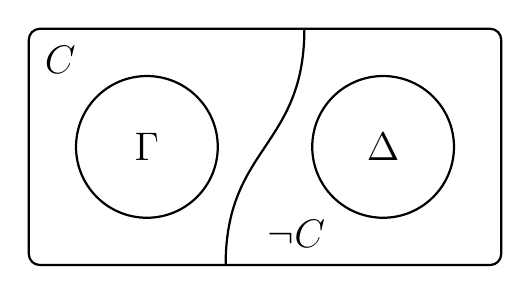
\begin{tikzpicture}[node distance=2cm, auto, thick]
    \draw [rounded corners] (0,0) -- (6,0) -- (6,3) -- (0,3) --  cycle;
    \draw (1.5,1.5) circle (0.9cm);
    \draw (4.5,1.5) circle (0.9cm);
    \path node at (1.5,1.5) {\Large $\Gamma$}; 
    \path node at (4.5,1.5) {\Large $\Delta$}; 
    \path node at (0.4,2.6) {\Large $\formula{C}$};
    \path node at (3.4,0.4) {\Large $\lnot \formula{C}$};
    \draw (2.5,0) .. controls (2.5,1.5) and (3.5,1.5) .. (3.5,3);
  \end{tikzpicture}
  \caption{$!C$ misahake $\Gamma$ lan $\Delta$}
  \ollabel{fig:sep}
\end{figure}


\begin{lem}\ollabel{lem:sep1}
Upamane $\Lang{L}_0$ iku basa kang ngemot saben
!!{constant}, !!{function} lan !!{predicate}
(saliyane $\doteq$) kang katon ing \emph{loro-lorone}
$\Gamma$ lan $\Delta$, lan $\Lang{L}'_0$ kawangun
kanthi nambah tanpa wates akeh !!{constant}s anyar
$\Obj c_n$ kanggo $n \ge 0$. Ing kene anyar tegese ora ana ing Gamma utawa Delta, ora mung ora ana ing basa irisan. Banjur yen
$\Gamma$ lan $\Delta$ ora bisa dipisahake ing
$\Lang{L}_0$, loro-lorone uga ora bisa dipisahake
ing $\Lang{L}'_0$.
\end{lem}

\begin{proof}
Kita nganggo bukti ora langsung: upamane kanggo
kontradiksi $\Gamma$ lan $\Delta$ bisa dipisahake
ing $\Lang{L}'_0$. Banjur $\Gamma \Entails
\Subst{!C}{c}{x}$ lan $\Delta \Entails \lnot
\Subst{!C}{c}{x}$ kanggo sawijining $!C \in
\Lang{L}_0$ (ing kene $c$ iku !!{constant} anyar---
yen ukara pamisah kang digawé saka $!C$
ngemot luwih saka siji
!!{constant} anyar kaya mangkono, carane padha).
Cathetan cakupan SOL6-F027: sadurunge konstanta anyar diganti variabel x kanggo nggawe formula asal, jeneng variabel kaiket ing ukara pamisah diganti yen perlu supaya ora ana kang diarani x. Kanthi iki, penggantian konstanta dening x ora dicekel dening kuantor, lan mung x kang dadi variabel bebas.
Cathetan koreksi sumber OLPL-112:
sing bisa ngemot konstanta anyar iku
ukara pamisah ing basa kang digedhekake,
dudu formula asal ing basa lawas.
Miturut kompaktitas, ana subhimpunan \emph{winates}
$\Gamma_0$ saka $\Gamma$ lan $\Delta_0$ saka
$\Delta$ kang njalari $\Gamma_0 \Entails
\Subst{!C}{c}{x}$ lan $\Delta_0 \Entails
\lnot \Subst{!C}{c}{x}$. Sebut $!G$ konjungsi
kabeh !!{formula}s ing $\Gamma_0$ lan $!H$
konjungsi kabeh !!{formula}s ing $\Delta_0$. Konjungsi saka himpunan kosong dianggep bener.
Banjur
\begin{align*}
  !G & \Entails \Subst{!C}{c}{x}, & !H  \Entails \lnot \Subst{!C}{c}{x}.
\end{align*}
Saka kang kapisan, kanthi Generalisasi, kita oleh
$!G \Entails \lforall[x][!C]$; saka kang kapindho,
kanthi kontraposisi, $\Subst{!C}{c}{x} \Entails
\lnot !H$, mula uga $\lforall[x][!C]
\Entails \lnot !H$. Cathetan koreksi sumber
OLPL-111: simbol delta ing sumber ora ditegesi;
ing langkah iki sing dimaksud yaiku konjungsi
kang diwenehi jeneng H. Kanthi kontraposisi maneh,
iki menehi $!H \Entails \lnot \lforall[x][!C]$.
Miturut monotonisitas,
\begin{align*}
  \Gamma &\Entails \lforall[x][!C], & 
  \Delta & \Entails \lnot \lforall[x][!C],
\end{align*}
mula $\lforall[x][!C]$ misahake $\Gamma$
lan $\Delta$ ing $\Lang{L}_0$.
\end{proof}

\begin{lem}\ollabel{lem:sep2}
Upamane $\Gamma \cup \{ \lexists[x][!S] \}$
lan $\Delta$ ora bisa dipisahake, lan $c$
iku !!{constant} anyar kang ora katon ing
$\Gamma$, $\Delta$, utawa $!S$. Banjur
$\Gamma \cup \{ \lexists[x][!S],
\Subst{!S}{c}{x} \}$ lan $\Delta$ uga
ora bisa dipisahake.
\end{lem}

\begin{proof}
Upamane kanggo kontradiksi $!C$ misahake
$\Gamma \cup \{ \lexists[x][!S],
\Subst{!S}{c}{x}\}$ lan $\Delta$, dene
$\Gamma \cup \{\lexists[x][!S] \}$ lan
$\Delta$ ora bisa dipisahake.
Cathetan koreksi sumber OLPL-113:
argumen eksistensial ing sumber nate
ditulis nganggo kurung kurawal;
ing kene nganggo wangun opsional
kang padha karo panganggone liyane.
Kita bedakake rong kasus:
\begin{enumerate}
\item $c$ ora katon ing $!C$: ing kasus iki,
  $\Gamma \cup \{\lexists[x][!S], \lnot!C \}$
  bisa dipenuhi (yen ora, $!C$ misahake
  $\Gamma \cup \{\lexists[x][!S] \}$ lan
  $\Delta$). Kahanan iki tetep bisa dipenuhi
  yen $\Subst{!S}{c}{x}$ ditambahake, mula
  $!C$ sejatine ora misahake
  $\Gamma \cup \{ \lexists[x][!S],
  \Subst{!S}{c}{x} \}$ lan $\Delta$.
\item $c$ katon ing ukara pamisah $!C$;
  saiki gunakake $!C$ kanggo formula asal
  kang, sawise substitusi, menehi ukara
  $\Subst{!C}{c}{x}$. Cathetan koreksi sumber
  OLPL-114: sumber nggunakake lambang C
  kanggo ukara pamisah lan formula sadurunge
  substitusi; rong panganggone dibedakake
  kanthi cetha ing kene. Kaya ing SOL6-F027, variabel kaiket ing ukara pamisah diganti jenenge luwih dhisik yen perlu, supaya penggantian c dening x ora nyebabake capture. Banjur kita duwe
  \[
  \Gamma \cup \{ \lexists[x][!S], \Subst{!S}{c}{x}\} \Entails \Subst{!C}{c}{x},
  \]
  mula $\Gamma, \lexists[x][!S] \Entails
  \lforall[x][(!S \lif !C)]$ miturut Teorema
  Deduksi lan Generalisasi, lan pungkasane
  $\Gamma \cup \{ \lexists[x][!S] \}
  \Entails \lexists[x][!C]$. Dene
  $\Delta \Entails \lnot \Subst{!C}{c}{x}$
  lan mula miturut Generalisasi
  $\Delta \Entails \lnot \lexists[x][!C]$.
  Mula $\Gamma \cup \{\lexists[x][!S] \}$
  lan $\Delta$ bisa dipisahake,
  sawijining kontradiksi.
\end{enumerate}
\end{proof}

\end{document}
